\documentclass[a4paper]{article}

\usepackage{minted} % Display Code
\usemintedstyle{friendly}
\setmintedinline{breaklines}
\usepackage{url} % Show URLs
\usepackage[utf8]{inputenc} % Encoding
\usepackage{chngcntr} % Counters
\counterwithin{figure}{section}
\usepackage{hyperref} % References
\usepackage{graphicx}

\renewcommand{\abstractname}{Executive Summary}

\title{Kademlia\\ \medskip{}
  \large{Sprint 0}
}

\author{
  August Eriksson~\thanks{augeri-5@student.ltu.se}\\
  Rasmus Bergström~\thanks{rasber-5@student.ltu.se}\\
  Robin Rubindal~\thanks{robrub-5@student.ltu.se}\\
}

\begin{document}

\maketitle
\newpage

\begin{abstract}
  Hello world! 
\end{abstract}


\newpage

\section{Introduction}
This is the project lab in the course D7024E taught at Luleå Tekniska Universitet (LTU), in which the students get to work with the distributed hash table (DHT) Kademlia by implementing a kademlia solution using containers to spin up a network. This project covers an implementation using google-go and docker.

\subsection{Architecture}
Below is a figure of the general architecture of a node before implementation, this will be updated during implementation.
\begin{figure}[ht]
\centering
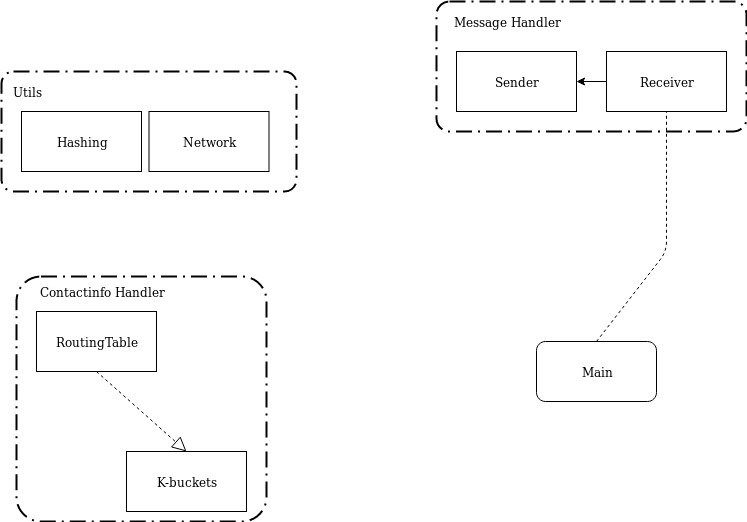
\includegraphics[width=\linewidth]{D7024E-architecture.jpg}
\caption{High-level architecture of a node in the kademlia implementation.}
\end{figure}

The main function starts the reciever listener as the 'busy-wait' loop so that the node does not terminate but awaits further instructions. The receiver then spawns new threads (goroutines) as needed to handle incoming instructions. The sender is used to send any messages to other nodes in the network. Utils handles any general functions such as hashing, a node getting its own IP, etc. While the routing table keeps records of a nodes k-buckets.

\newpage

\section{Sprint 1 Plan}
After a discussion we estimated that we will complete the mandatory objectives for this project during the first sprint. For the backlog, see our Github.\footnote{\href{https://github.com/JRasmusBm/D7024E_Lab_Kademlia}{https://github.com/JRasmusBm/D7024E\_Lab\_Kademlia}}\\

\textbf{Networking:} A node shall be able to ping any other node, a node should be able to join the Kademlia network and a node shall be able to find any other node in the Kademlia network.\\

\textbf{Objects:} Any node must be able to upload an object (key:val pair) that will be stored on appropriate nodes according to the kademlia principle. Any node must be able to find and download any object stored on at least one node of the kademlia network.\\

\textbf{CLI:} Each node must be able to execute the following commands: put, get and exit. Exit terminates the node, get takes a hash as its arguement and outputs the node and the value sought if it exists. Put takes a value as an arguement and outputs the hash if uploaded successfully.\\

\textbf{Testing:} At least a 50\% testing coverage of the implementation.\\

\textbf{Containers:} A network of at least 50 nodes must be spinned up by containers where each node is a seperate container.\\

\bibliographystyle{plain}
\bibliography{sources}

\end{document}
